\documentclass[12pt]{article}

\usepackage{graphicx}
\usepackage{url}
\usepackage{amsmath}
\usepackage[cm]{fullpage}
\usepackage{calc}
\usepackage{subfig}

\title{\textbf{Wireless and Mobile Computing, Assignment 6}}
\author{Marcel Mohler & Thomas Richner}
\begin{document}
\maketitle

\section{Setup}

We use a scenario where one station is a receiver and two stations send traffic to this receiver. Both sending stations make use of two ACs, hence send two data flows to the receiving station. The receiver therefore has four incoming flows.

\begin{figure}[h!]
\centering
\includegraphics[width=160mm]{img/setup.png}
\caption{setup, receiver station and two sending stations \label{fig:setup}}
\end{figure}


\section{Algorithm Design}

\subsection{Design Goals}

\subsection{Implementation}

\section{Evaluation}

\subsection{Measurements}

\subsection{Discussion & Conclusion}


\section{Feedback}

\begin{description}
  \item[Difficulty] \hfill \\ appropriate
  \item[Clarity] \hfill \\ 
  \item[Time Spent] \hfill \\ 5h
  \item[Conclusion] \hfill \\ Jemula...
\end{description}

\end{document}
